\documentclass[tikz,border=5]{standalone}
\usepackage{amsmath}
\usepackage{amssymb}
\usepackage{tikz}
\usetikzlibrary{calc,fit,patterns,decorations.markings,matrix,3d}

\begin{document}

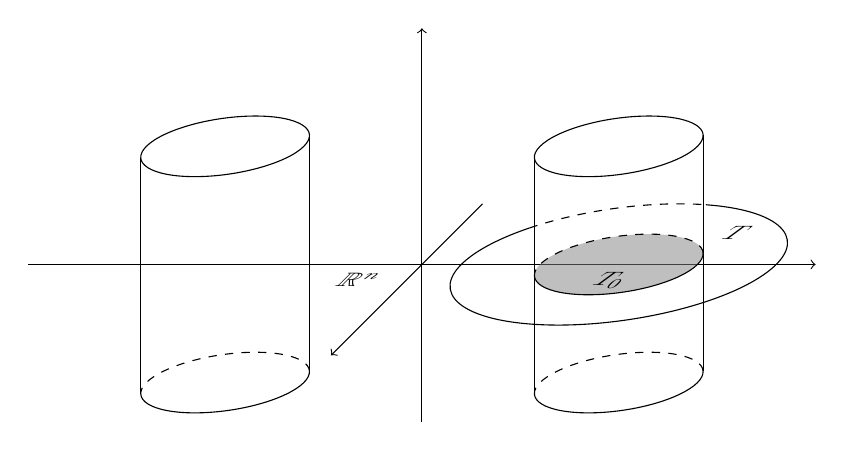
\begin{tikzpicture}[scale=1]
\def\Anglei{-67.5}
\def\Angleii{233}
\def\Angleiii{170}

\draw[thin,->] (-5,0) -- (5,0);
\draw[thin,->] (0,-2) -- (0,3);

%Zylinder
\begin{scope}[canvas is zx plane at y=0]
\coordinate (circmb) at ( $ (0,2.5) + (\Angleii:2cm) $ );
\coordinate (circma) at ( $ (0,2.5) + (\Angleiii:2cm) $ );
\draw[dashed] (circmb) arc [start angle=\Angleii,end angle=\Angleiii,radius=2cm];
\draw (circma) arc [start angle=\Angleiii,end angle=\Angleii-360,radius=2cm];
\fill[fill=gray,opacity=0.5] (0,2.5) circle (1cm);

\coordinate (circm1) at ( $ (0,2.5) + (\Anglei:1cm) $ );
\coordinate (circm2) at ( $ (0,2.5) + (180+\Anglei:1cm) $ );

\draw (circm1) arc [start angle=\Anglei,end angle=180+\Anglei,radius=1cm];
\draw[dashed] (circm2) arc [start angle=180+\Anglei,end angle=360+\Anglei,radius=1cm];

\draw[->] (-2,0) -- (3,0);
\end{scope}

\begin{scope}[canvas is zx plane at y=1.5]
\path (0,2.5) circle (1cm);
\coordinate (circ1a) at ( $ (0,2.5) + (\Anglei:1cm) $ );
\coordinate (circ1b) at ( $ (0,2.5) + (180+\Anglei:1cm) $ );
\end{scope}

\begin{scope}[canvas is zx plane at y=-1.5]
\path (0,2.5) circle (1cm);
\coordinate (circ2a) at ( $ (0,2.5) + (\Anglei:1cm) $ );
\coordinate (circ2b) at ( $ (0,2.5) + (180+\Anglei:1cm) $ );
\end{scope} 

\begin{scope}[canvas is xy plane at z=0]
\draw (circ1a) -- (circ2a);
\draw (circ1b) -- (circ2b);
\end{scope}

\begin{scope}[canvas is zx plane at y=1.5]
\draw (0,2.5) circle (1cm);
\end{scope}

\begin{scope}[canvas is zx plane at y=-1.5]
\draw (circ2a) arc [start angle=\Anglei,end angle=180+\Anglei,radius=1cm];
\draw[dashed] (circ2b) arc [start angle=180+\Anglei,end angle=360+\Anglei,radius=1cm];
\end{scope} 

\begin{scope}[canvas is zx plane at y=1.5]
\path (0,-2.5) circle (1cm);
\coordinate (circ3a) at ( $ (0,-2.5) + (\Anglei:1cm) $ );
\coordinate (circ3b) at ( $ (0,-2.5) + (180+\Anglei:1cm) $ );
\end{scope}

\begin{scope}[canvas is zx plane at y=-1.5]
\path (0,-2.5) circle (1cm);
\coordinate (circ4a) at ( $ (0,-2.5) + (\Anglei:1cm) $ );
\coordinate (circ4b) at ( $ (0,-2.5) + (180+\Anglei:1cm) $ );
\end{scope} 

\begin{scope}[canvas is xy plane at z=0]
\draw (circ3a) -- (circ4a);
\draw (circ3b) -- (circ4b);
\end{scope}

\begin{scope}[canvas is zx plane at y=1.5]
\draw (0,-2.5) circle (1cm);
\end{scope}

\begin{scope}[canvas is zx plane at y=-1.5]
\draw (circ4a) arc [start angle=\Anglei,end angle=180+\Anglei,radius=1cm];
\draw[dashed] (circ4b) arc [start angle=180+\Anglei,end angle=360+\Anglei,radius=1cm];
\end{scope} 

\begin{scope}[every node/.append style={
xslant=1,sloped}
]
\node at (2.4,-.2) {\scalebox{1}[.7]{$T_0$}};
\node at (4,.4) {\scalebox{1}[.7]{$T$}};
\node at (-.8,-.2) {\scalebox{1}[.7]{$\mathbb{R}^n$}};
\end{scope}
\end{tikzpicture}

\end{document}